\chapter{SISTEMAS EXPERTOS Y PROYECTO MIA}

%Contadores y formato para numeracion de elementos
\renewcommand{\thefootnote}{\arabic{footnote}}
\renewcommand{\theequation}{\arabic{chapter}-\arabic{equation}}
\renewcommand{\thefigure}{\arabic{chapter}.\arabic{figure}}
\renewcommand{\figurename}{Figura}
\renewcommand{\tablename}{\textbf{Tabla}}
\renewcommand{\thetable}{\textbf{\arabic{chapter}-\arabic{table}}}
\stepcounter{definitionN}
\stepcounter{exampleN}
\stepcounter{tableN}
\stepcounter{footN}
\stepcounter{algorithmN}
\providecommand{\abs}[1]{\lvert#1\rvert}
\providecommand{\norm}[1]{\lVert#1\rVert}
%%%agregue el paquete caption
\newpage

%\title{SISTEMAS EXPERTOS Y PROYECTO MIA}\label{sec:intro}
En este capítulo se presentan los principales detalles que se deben tener en cuenta en la construcción de un sistema experto.  El tema tiene especial importancia en el marco del proyecto MIA debido a que, por ejemplo, el simulador prototipo que se ha construido, arroja gran cantidad de información y suministra algunas herramientas que permiten su análisis; sin embargo, ese análisis debe estar en manos de un conjunto de expertos, bien sean humanos o automático o bien una mezcla de ambas.  \\
La ingeniería que hay detrás de la construcción de un sistema de esta naturaleza es muy avanzada pero en esta rama de la ingeniería  aún hay mucho sin descubrir o inventar.  Por esa razón, es bueno tener una dosis de optimismo en las reales posibilidades de este tipo de sistemas pero, a la vez, tener las suficientes precauciones debido a que la herramienta por sí sola no puede obtener resultados aceptables.  El tratamiento temático de este capítulo está inspirado en (Peter \& Russell, 1989), (Rolston, Gama, \& Ziskiend, 1990) y (Ortiz Triviño, 2009).
\section{	DEFINICIÓN DE UN SISTEMA EXPERTO}
De acuerdo con (Rolston et al., 1990) un SE es un software cuya finalidad es  solucionar problemas complicados que de otra manera exigirán ampliamente la pericia humana. Para lograr esto, se simula el proceso de razonamiento humano mediante la aplicación específica de conocimientos y de inferencias. En su estructura se pueden encontrar algunos subsistemas que son comunes a todo sistema experto:
\begin{itemize}
\item 	Conocimiento específico a partir del campo de interés, por ejemplo, en medicina, conducción, petróleos, etc.
\item Módulo para realizar búsqueda,
\item 	Un componente para análisis heurístico,
\item	Un módulo que le permita tener la habilidad para inferir nuevos conocimientos a partir de conocimientos ya existentes,
\item 	Un módulo que le permita  procesar símbolos más allá de los números.
\item 	Un módulo que lo dote de la capacidad para explicar su propio razonamiento.
\end{itemize}
\section{	ANÁLISIS DE LA SOLUCIÓN PRÁCTICA DE PROBLEMAS}
Uno de los primeros pasos cuando se empieza a pensar en la necesidad de la construcción de un sistema experto está en delimitar muy bien el ámbito sobre el cual ese sistema será realmente experto y si, luego de un cuidadoso análisis de costo beneficio, se justifica la ejecución de su construcción.  Los alcances y las limitaciones de dicho sistemas son fundamentales en la toma de la decisión.\\
Experiencia y conocimiento son dos propiedades que todo sistema experto debe exhibir.  En cuanto a la segunda de ellas, el conocimiento, es ampliamente aceptado, véase (Peter \& Russell, 1989), que la utilidad de un sistema experto se debe más al conocimiento  en el área específica que al mismo desempeño genérico del experto. 
\section{ARQUITECTURA TÍPICA  DE UN SISTEMA EXPERTO}
Alguno de los componentes del conocimiento que hacen posible producir la habilidad artificial de un  experto humano en su desempeño son las siguientes: 
\begin{itemize}
    \item 	Los \textbf{Hechos}. Proposiciones que relacionan algunos elementos de la realidad con referencia al área específica. Por ejemplo, el derrame de petróleo deteriora el ambiente.  Frecuentemente, los hechos son capturados a través de sensores que llevan la información desde el contexto al interior del experto. 
    \item 	Las \textbf{Reglas de procedimiento} . Reglas bien definidas e invariables que describen secuencias fundamentales de eventos y relaciones relativas al área. Por ejemplo, siempre apague el vehículo antes de intentar suministrarle gasolina. Si el altímetro señala el nivel de vuelo, el medidor de la velocidad vertical debe marcar cero.
    \item 	Las \textbf{Reglas heurísticas}. En ellas se consigna la experiencia. Son reglas generales en forma de opiniones o reglas em\\píricas que sugieren procedimientos que se pueden seguir cuando no existen disponibles reglas de procedimiento invariables. Dichas reglas son, de acuerdo con (Rolston et al., 1990),  aproximadas y han sido generalmente producidas por un experto a través de años de experiencia. Por ejemplo, un piloto de avión, puede saber de acuerdo con su experiencia que es mejor intentar un aterrizaje de emergencia bajo condiciones controladas que volar en condiciones desconocidas.  Lo realmente interesante e importante de ello es que el uso de heurísticas contribuye grandemente a la potencia y flexibilidad de los SE y tiende a distinguirlos aún más del software tradicional.
\end{itemize}
Hay, sin embargo, otras formas específicas de conocimientos, de esta manera, un experto posee un modelo conceptual general del área específica y un esquema global para hallar una solución así como también una estructura de preferencias. Estas le permiten una “visión global”.  En conjunto, ellas conforman la infraestructura básica para la aplicación por parte del experto de conocimientos detallados.   \\
\begin{figure}[H]
\centering
\captionsetup{justification=centering,margin=2cm}
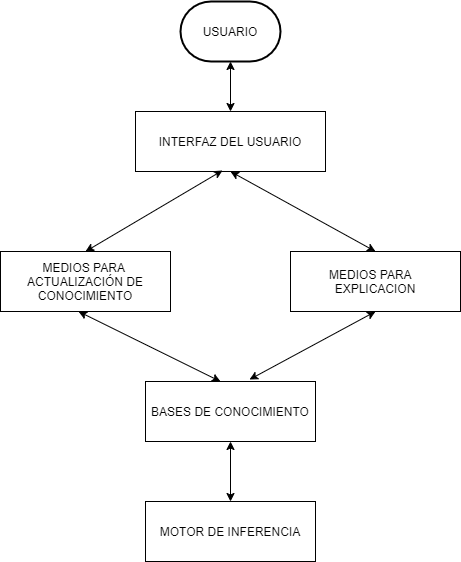
\includegraphics[scale=0.4]{chapters/chapter10/figures/1-1.png}
\caption{Arquitectura típica de sistemas expertos (Adaptado de (Rolston et al., 1990)).}
\label{fig:10-1}
\end{figure}

Los SE contemporáneos emplean una gran variedad de arquitecturas específicas en sus configuraciones, principalmente porque una arquitectura es más aplicable que otra cuando se considera una aplicación dada. Actualmente de acuerdo con (Rolston et al., 1990) las investigaciones en el tema no han llegado a una conclusión definitiva; al contrario, subsiste un considerable debate al respecto.\\
Sin embargo, en cuanto a la esencia de un SE si parece existir un consenso.  A pesar de las diferencias significativas, la mayoría de las arquitecturas tienen muchos componentes en común. La Figura \ref{fig:10-1} muestra una arquitectura general con los componentes típicos. En lo que sigue de este documento se darán algunos de talles adicionales de los módulos presentados en esa gráfica general.\\
\subsection{El usuario}

Existen varios tipos de usuario, o varios roles asociados con la interacción con un SE.  Los más comunes para (Rolston et al., 1990) son los siguientes:
\begin{itemize}
    \item \textbf{Verificador}	. El usuario intenta comprobar la validez del desempeño del sistema.
     \item 	\textbf{Tutor}. El usuario da información adicional al sistema o modifica el conocimiento que ya está presente en el sistema.
     \item 	\textbf{Alumno}. El usuario busca rápidamente desarrollar pericia personal relacionada con el área específica mediante la recuperación de conocimientos organizados y condensados en el sistema.
     \item \textbf{Cliente}	. El usuario aplica la pericia del sistema a tareas específicas reales.
\end{itemize}
El reconocimiento de las caracterizaciones, reconociendo varios tipos posibles de interacción, anteriores contrasta con la percepción de un simple papel (el cliente) de los sistemas tradicionales de software.
\subsection{	Facilidades de interfaz con el usuario}
La comunicación desde el ambiente hacia el interior del SE y desde el SE hacia el ambiente son características fundamentales.  Un SE no es un sistema aislado, todo lo contrario, debe compenetrarse con su entorno. Las facilidades de interfaz con el usuario y con el contexto deben aceptar información del usuario y traducirla a una forma aceptable para el resto del sistema o aceptar información proveniente del sistema y convertirla a una que el usuario pueda entender. No solamente se trata de una sofisticada interfaz gráfica.  Esta comunicación va mucho más allá. Actualmente, por ejemplo, en este aspecto se incluyen las redes de sensores y actuadores que le permiten al SE Artificial de acuerdo con lo que esta ocurriendo afuera de él.\\
Idealmente, esta facilidad se compone de un sistema procesador de lenguaje natural que acepta y  devuelve esencialmente información en la misma forma como es aceptada u ofrecida por una persona experta. En la actualidad existen sistemas que reproduzcan las capacidades del  lenguaje humano con destacado éxito, y también existen muchos otros que han producido impresionantes resultados mediante la utilización de subconjuntos restringidos del lenguaje.\\
Las facilidades de interfaz del usuario a menudo se diseñan para reconocer el modo en que el usuario está operando, su nivel de pericia, y la naturaleza de la transacción. La comunicación con un SE debe ser tan natural como sea posible, toda vez que el sistema trata de sustituir el desempeño humano.
\subsection{	Sistema de almacenamiento y generación de conocimiento}
El almacenamiento de conocimiento, el cual es de mayor complejidad y abstracción que los simples datos o la información, consta de una base de conocimientos y un motor de inferencia. Es el corazón de un SE. La función de este sistema consiste en almacenar confiablemente los conocimientos del experto, para recuperarlos e inferir nuevos conocimientos cuando se requiera.\\
\textbf{Base de conocimientos}. La base de conocimientos representa un depósito de las primitivas del conocimiento (por ejemplo, hechos fundamentales, reglas de procedimientos y heurísticas) disponibles para el sistema. Como se dijo anteriormente, el conocimiento guardado en la base, establece la capacidad del sistema para actuar como un experto.\\
En general, el conocimiento se almacena en forma de \textbf{hechos} y de \textbf{reglas}, pero los esquemas específicos empleados para almacenar la información varían grandemente. El diseño de este esquema de representación de conocimientos afecta el diseño del motor de inferencia, el proceso de actualización del conocimiento, el proceso de explicación y la eficiencia global del sistema.\\
Todo lo anterior conduce a pensar que la selección del esquema de representación del conocimiento es una de las decisiones más críticas en el diseño de un SE.\\
Inferencia de conocimientos. De acuerdo con (Peter \& Russell, 1989) la ingeniería de conocimientos es el proceso de adquirir el conocimiento del área específica y estructurarlo en la base de conocimientos. La Figura \ref{fig:10-2} ilustra cómo se da típicamente el proceso. Los conocimientos pueden conseguirse de una variedad de fuentes, por ejemplo redes de sensores conectados al sistema experto, incluyendo la documentación y los sistemas de información  computacional existentes, la mayor parte de él, debe obtenerse de personas experta. El conocimiento suministrado por el experto, por lo general estará en forma tal que sea orientado hacia el tema del área.
\begin{figure}[H]
\centering
\captionsetup{justification=centering,margin=2cm}
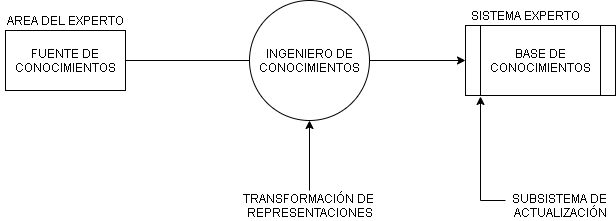
\includegraphics[scale=0.6]{chapters/chapter10/figures/1-2}
\caption{Ingeniería de conocimientos (Adaptado de (Hidalgo, 1996)).}
\label{fig:10-2}
\end{figure}
Surge de ahí un rol indispensable a tener en cuenta en el sistema MIA: El ingeniero de conocimiento (IC) quien es la persona que obtiene los conocimientos del área del experto y las transporta a la base de conocimientos. La Figura \ref{fig:10-4} bosqueja la labor del ingeniero del conocimiento. En razón de que un sistema experto requiere que los conocimientos en la base de conocimientos se guardan de acuerdo con las normas de representación de conocimientos del sistema, el IC debe transformar la representación del conocimiento como parte del proceso de transporte.\\
Para adquirir el reconocimiento necesario, el IC primero debe establecer una comprensión global del área, formar un diccionario mental de los términos y jerga esenciales del área y desarrollar una comprensión básica de los conceptos claves. Luego debe condensar los conocimientos sucintos a partir de la información suministrada por el experto.\\
La función de adquisición de conocimientos en comúnmente, el aspecto de mayor dificultad en la construcción de SE lo cual enfatiza aun más la importancia del IC.. Esto se debe principalmente al hecho de que el proceso requiere comunicaciones humanas ampliadas, entre el experto en el área y el IC y en consecuencia enfrenta los problemas asociados con esta actividad. Por tanto, según (Rolston et al., 1990)  el proceso de adquisición del conocimiento no está bien entendido ni bien definido. Si el proceso mismo de desarrollo de un SE se visualizara como un área para expertos, el conocimiento asociado con el procedimiento de adquisición sería considerado como heurístico.\\
\begin{figure}[H]
\centering
\captionsetup{justification=centering,margin=2cm}
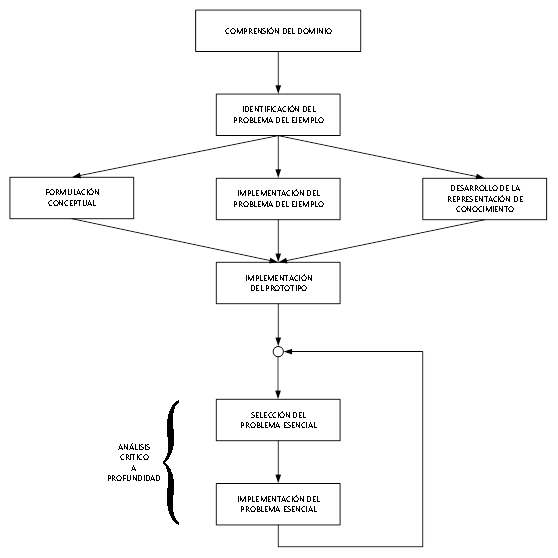
\includegraphics[scale=1]{chapters/chapter10/figures/10-3}
\caption{Identificación de problema (Tomado de (Rolston et al., 1990)).}
\label{fig:10-3}
\end{figure}
\textbf{Motor de indiferencia}. Los SE deben, por su naturaleza, tratar flexiblemente con situaciones dinámicas y estocásticas. La capacidad para adaptarse y  responder ante situaciones cambiantes depende de la habilidad para inferir nuevos conocimientos a partir de conocimientos existentes.  El ejemplo proporcionado por (Rolston et al., 1990) ilustra muy bien esta idea. Considere los dos hechos básicos siguientes:
\begin{enumerate}
\item Todos los animales respiran oxígeno.
\item Todos los perros son animales.
\end{enumerate}
Se puede inferir un nuevo hecho, “todos los perros respiran oxígeno” a partir de los dos hechos anteriores. Para responder a una situación dada, un SE debe aplicar el conocimiento apropiado. La aplicación de conocimientos apropiados implica que los conocimientos requeridos fueron o identificados como conocimientos existentes en la base de conocimientos o inferidos a partir de estos.\\
Lo discutido hasta este momento sirve de justificación para la afirmación de(Peter \& Russell, 1989) según la cual el proceso de buscar los conocimientos apropiados y a partir de estos deducir nuevos conocimientos constituye un elemento clave del procesamiento de un sistema experto.  Por lo tanto, a diferencia de postulados de la construcción de otros tipos de sistemas computacionales como los sistemas de información o las bases de datos, en un SE es deseable (y probablemente necesario) almacenar el conocimiento adquirido aunque éste pueda ser nuevamente inferido de las reglas primitivas.\\
Una de las mayores dificultades asociadas con la operación a partir de las primitivas es el hecho que, aun unos pocos elementos individuales (tales como, primitivas)  se puedan combinar dentro de un número muy grande de combinaciones únicas. El número de posibilidades a partir de un conjunto grande de elementos, rápidamente se convierte en una cifra astronómica. Este problema se conoce como explosión combinatoria. \\
El motor de inferencia es el software que ubica los conocimientos e infiere nuevos usando la base de conocimientos. El paradigma del motor de inferencia es la estrategia de búsqueda que se emplea para producir el conocimiento demandado. Varios paradigmas diferentes se emplean en un SE, pero la mayoría de ellos se basan en dos conceptos fundamentales: encadenamiento hacia atrás (o retroencadenamiento) que es un proceso de razonamiento descendente, que se inicia a partir de los objetivos deseados y trabaja hacia atrás en dirección a las condiciones pre-requisito, o el encadenamiento hacia adelante (o encadenamiento frontal) que es un procesamiento de razonamiento ascendente que se inicia con condiciones conocidas y trabaja hacia adelante para alcanzar los objetivos deseados.\\
Una conclusión sobre esta discusión la proporciona (Peter & Russell, 1989).  Ellos indican que a selección del paradigma de inferencia considerando la explosión combinatoria, influye fuertemente en el desempeño global de un SE y dependerá del ámbito específico del problema que deba asignársele al experto. \\
\subsection{Actualización de conocimientos}
\begin{figure}[H]
\centering
\captionsetup{justification=centering,margin=2cm}
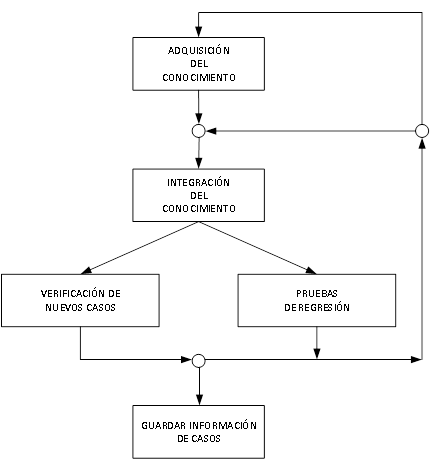
\includegraphics[scale=0.8]{chapters/chapter10/figures/10-4}
\caption{Implementación del conocimiento básico (Adaptado de (Rolston et al., 1990)).}
\label{fig:10-4}
\end{figure}
Como se ha insistido, la base de conocimiento es una reflexión cuidadosa del área en el momento en que el sistema se pone en servicio. Pero en muchas áreas complejas el conocimiento crece y cambia constantemente por lo cual la base de conocimientos de bebe modificar en el mismo sentido. Para llevar a cabo tales actualizaciones se emplean la facilidad para actualización de conocimientos. Este módulo puede tomar una de tres formas fundamentales (Rolston et al., 1990), según como se describe a continuación.\\
La primera forma, y también la más primitiva, es la actualización manual de conocimientos. En este caso la actualización se lleva a cabo por un IC quien interpreta la información ofrecida por un experto en el área y actualiza la base de conocimientos mediante el uso de un sistema limitado de actualización. \\
En la segunda forma, mucho más ambiciosa y prometedora, el experto en el área ingresa directamente el conocimiento revisado sin la mediación de un ingeniero  de conocimientos. En este caso el sistema de actualización de conocimientos debe ser mucho más elaborado.\\
En la tercera forma, donde se encuentra la frontera del conocimiento en este campo, el sistema genera nuevos conocimientos en forma automática y se basa en generalizaciones deducidas de experiencias anteriores. El sistema aprende nominalmente de la experiencia y se espera que el mismo sistema se actualice. Este proceso, se han logrado algunos buenos avances pero que aún está muy lejos de excelentes resultados, es tema de mucha investigación. La habilidad para aprender es un componente importante de la inteligencia y al ofrecer completamente esta potencialidad mejoraría las capacidades de un SE.\\
De esta manera, de forma ideal, puede afirmarse que en un SE ideal, el motor de inferencia nunca debería necesitar de modificaciones. En consecuencia, todas las mejoras al sistema de conocimientos se implementan mediante la expansión de la base de conocimientos. Sin embargo, según (Rolston et al., 1990), es raro que sea posible el asegurar una completa independencia de la base de conocimientos y del motor de inferencia.\\
\subsection{	Sistema de explicaciones}
Además de lograr simplemente una conclusión cuando se enfrenta un problema complicado, un experto también debe ser capaz de explicar lo cual implica comprender, hasta cierto punto, el razonamiento que conduce a dicha conclusión. Un SE debe diseñarse para brindar una facultad semejante. Esta es una potencialidad que generalmente está ausente en los sistemas tradicionales de computación pero que conforme pasa el tiempo se van convirtiendo en parte de las actuales soluciones informáticas (no necesariamente un SE).\\
Comúnmente, análogo a como se demuestra un teorema en el campo de las matemáticas,  la explicación consiste en una identificación de los pasos en el proceso de razonamiento y de una justificación de cada uno de ellos.  El implementar esta potencialidad para comunicar esta información, constituye esencialmente un subconjunto del problema del procesamiento de lenguaje natural. El sistema debe acceder a un registro de los conocimientos que se emplearon en el procesamiento, basándose en el esquema de representación de la base de conocimientos y traducirlo a una forma que sea aceptable y (principalmente) comprensible para el usuario.\\
Por lo tanto,  la credibilidad que se le concede a un SE, como ocurre también entre los humanos, depende de la habilidad del SE para explicar su propio proceso de razonamiento.  Reiterando, una persona experta también puede ser capaz de explicar sus razonamientos en forma adecuada al nivel de experiencia del que escucha. Un gerente de perforación de un pozo petrolero podría explicar a sus superiores que la perforación se ha cancelado debido a que los resultados de un reciente estudio sobre el terrero indica que la probabilidad de que ahí haya petróleo es de apenas 0.0005. \\
En consecuencia, para proporcionar los niveles críticos de explicación, el sistema debe identificar el nivel de conocimientos del usuario y entender cómo adaptar la explicación para acoplarla apropiadamente. Aún hoy en día con los desarrollos alcanzados, las facilidades de explicación en varios sistemas actuales se limitan a listar simplemente las reglas que se utilizaron durante la ejecución y son incapaces de justificar la razón.\\
\section{	LENGUAJES DE PROGRAMACIÓN PARA SISTEMAS EXPERTOS}
Por lo general, al desarrollar sistemas expertos la programación se centra en los temas de inferencia y búsqueda heurística y depende esencialmente de la manipulación de símbolos: series de caracteres. Los lenguajes de programación tradicionales para estas tareas son por excelencia LISP y PROLOG.  Estos lenguajes son los más empleados en la construcción de SE, aunque muchos lenguajes convencionales específicamente C, JAVA, Python entre otros, han cobrado mucha relevancia en el mundo contemporáneo.\\
El procesamiento simbólico es importante en SE, debido a que las primitivas de conocimiento en una base de conocimientos y las relaciones entre las primitivas de conocimientos, se almacenan mediante el uso de representaciones simbólicas. Es útil que los lenguajes de programación para SE puedan tratar libremente con ``cosas``, sin estar comprometido con la composición de dichas cosas.\\
\begin{figure}[H]
\centering
\captionsetup{justification=centering,margin=2cm}
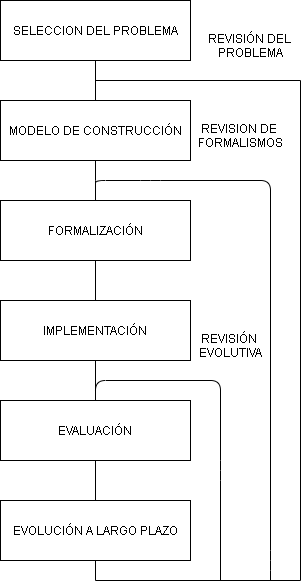
\includegraphics[scale=0.4]{chapters/chapter10/figures/1-5}
\caption{Ciclo de vida en la construcción de un SE (Adaptado de (Rolston et al., 1990).}
\label{fig:10-5}
\end{figure}
Una idea prometedora y no descabellada pero eso si compleja consiste en desarrollar primero el lenguaje de programación sobre el cual se desarrollará todo el sistema.  Esto debido a que ni LIST ni PROLOG  cuentan con herramientas adecuadas para manejar e inferir conocimiento de tipo difuso como fue propuesto para este proyecto.  Por esa razón puede pensarse en construir la herramienta (lenguaje de programación) con base en el cual se edificará la solución propuesta.\\
Cabe destacar que para lograrlo no solamente se debe emplear el paradigma de programación lógico sino que es fundamentar incorporar las capacidades de manejo de Objeto, eventos, programación distribuida, etc. También vale decir que no se trata de evitar el uso de lenguajes de programación que han mostrado sus grandes virtudes en el desarrollo de soluciones informáticas contemporáneas sino, más bien, construir un complemento de ellas para el caso particular en el que las herramientas existentes son débiles.\\
\section{ETAPAS DE DESARROLLO DE SISTEMAS EXPERTOS}
El proceso de desarrollo de SE, descrito en la Figura \ref{fig:10-5}, consiste de varias etapas básicas que son similares a las etapas típicas del ciclo de vida en ingeniería de software. La construcción de un SE es la construcción de un software y en ese sentido, las metodologías de desarrollo de aplicaciones es válida para este caso; sin embargo, el desarrollo de un SE tiene particularidades que lo diferencial del resto de programas por esa razón se hace necesario adaptar las metodologías y tener el debido cuidado al momento de emplearlas para este tipo de soluciones.\\
En general, estas etapas de construcción de un SE son (Rolston et al., 1990): \textbf{identificación del problema, construcción de un prototipo, formalización, implantación, evaluación y evolución a largo plazo}. La primera la  tarea en el desarrollo de cualquier SE, cuya estructura se esboza en Figura \ref{fig:10-3}, es establecer que el problema propuesto sea apropiado y requiera ser solucionado mediante un SE. Si el problema en consideración se puede describir en términos de definiciones y algoritmos explícitos, probablemente sea preferible desarrollar la solución de programación tradicional. Si el problema no está bien identificado o demanda amplio criterio humano (toma de decisiones de impacto ambiental y estabilidad financiera de las compañías, fijar políticas y establecer estrategias o juzgar la bondad en el bienestar de alguna estrategia), es probable que sea apropiado (aunque hay que tener cuidado) complejo para un SE.
\begin{figure}[H]
\centering
\captionsetup{justification=centering,margin=2cm}
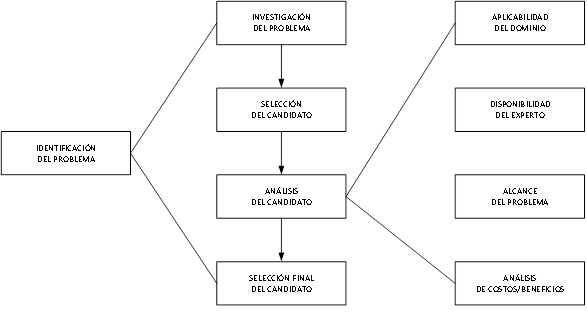
\includegraphics[scale=0.8]{chapters/chapter10/figures/10-6}
\caption{Identificación de problema}
\label{fig:10-6}
\end{figure}
Una vez el problema se ha seleccionado, se construye un prototipo pequeño para ayudar en la comprensión del problema completo y estimar la tarea de la construcción de la solución total. El siguiente paso en el proceso de desarrollo, es formalizar el enunciado del problema y diseñar completamente el SE.  En este punto del proceso se implementan y se interconectan todos los módulos de la Figura \ref{fig:10-7}.  Después de la formalización se realiza la implantación. Esto consiste principalmente de un ciclo continuo de adquisición de conocimientos, actualización de la base de conocimientos y pruebas.  Aquí es importante la selección de las herramientas de desarrollo que debería incluir la construcción de un lenguaje de programación para tal fin.\\
Por último, en la fase de evaluación, que sigue a la implantación, la estimación de la proximidad del sistema al desempeño experto. Después de la evaluación y entrega, el SE entra a un periodo de evolución a largo plazo. Durante este periodo el sistema continúa incrementado su competencia (según la experiencia que se vaya logrando con su empleo) y se revisa como respuesta a los cambios en los conocimientos del área. \\
Evidentemente es un sistema de alta complejidad pero, de la misma manera, puede decirse que la ingeniaría colombiana está preparada para su implementación.  Se requiere voluntad, tiempo suficiente y  recursos que permitan su realización.\\
\begin{figure}[H]
\centering
\captionsetup{justification=centering,margin=2cm}
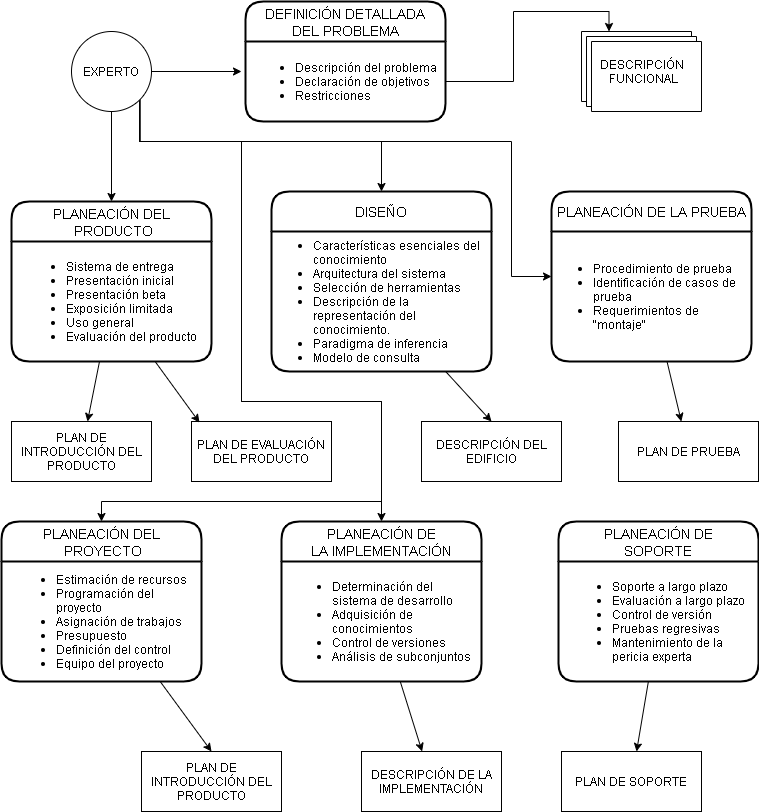
\includegraphics[scale=0.4]{chapters/chapter10/figures/1-7}
\caption{Formalización del SE (Adaptado de (Rolston et al., 1990)).}
\label{fig:10-7}
\end{figure}
Una observación que vale la pena subrayar antes de terminar el capítulo es que el sistema de control difuso que se propone en la capa más alta de toda la evolución del proyecto MIA, es, en sí mismo, un sistema experto.\\

